%%%%%%%%%%%%%%%%%%%%%%%%%%%%%%%%%%%%%%%%%%%%%%%%%%%%%%%%%%%%%%%%%%%%%%%%%%%%%%%%
% ISE Lab -- Topic
% Giovanni Ciatto
% Alma Mater Studiorum - Università di Bologna
% mailto:giovanni.ciatto@unibo.it
%%%%%%%%%%%%%%%%%%%%%%%%%%%%%%%%%%%%%%%%%%%%%%%%%%%%%%%%%%%%%%%%%%%%%%%%%%%%%%%%
%\documentclass[handout]{beamer}\mode<handout>{\usetheme{default}}
%
\documentclass[presentation]{beamer}\mode<presentation>{\usetheme{AMSBolognaFC}}
%\documentclass[handout]{beamer}\mode<handout>{\usetheme{AMSBolognaFC}}
%%%%%%%%%%%%%%%%%%%%%%%%%%%%%%%%%%%%%%%%%%%%%%%%%%%%%%%%%%%%%%%%%%%%%%%%%%%%%%%%
\usepackage{ise-lab-common}
\usepackage{ise-lab-ske}
% version
\newcommand{\versionmajor}{0}
\newcommand{\versionminor}{1}
\newcommand{\versionpatch}{1}
\newcommand{\version}{\versionmajor.\versionminor.\versionpatch}
%%%%%%%%%%%%%%%%%%%%%%%%%%%%%%%%%%%%%%%%%%%%%%%%%%%%%%%%%%%%%%%%%%%%%%%%%%%%%%%%
\title[\currentLab{} -- XAI via SKE]{
    eXplainable Artificial Intelligence via Symbolic Knowledge Extraction
}
%
\subtitle{\courseName{} / Module \moduleN{} (\courseAcronym)}
%
\author[\sspeaker{\gcShort}]{\speaker{\gcFull} \\ \gcEmail}
%
\institute[\disiShort, \uniboShort]{\disi{} (\disiShort)\\\unibo}
%
\date[A.Y. \academicYear{} (v.\ \version)]{Academic Year \academicYear{}\\(version \version)}
%
%%%%%%%%%%%%%%%%%%%%%%%%%%%%%%%%%%%%%%%%%%%%%%%%%%%%%%%%%%%%%%%%%%%%%%%%%%%%%%%%
\begin{document}
%%%%%%%%%%%%%%%%%%%%%%%%%%%%%%%%%%%%%%%%%%%%%%%%%%%%%%%%%%%%%%%%%%%%%%%%%%%%%%%%

%/////////
\frame{\titlepage}
%/////////

%%===============================================================================
\section*{Outline}
%%===============================================================================
%
%%/////////
\frame[c]{\tableofcontents[hideallsubsections]}
%%/////////

%===============================================================================
\section{Motivation \& Context}
%===============================================================================

\begin{frame}{Context}
    \begin{itemize}
        \item Pervasive \alert{adoption} of AI- and ML-powered solution world-wide
        %
        \begin{itemize}
            \item for \alert{automation} and decision support
        \end{itemize}
        
        \vfill
        
        \item[$\Rightarrow$] Several activities are (partially?) \alert{delegated} to intelligent machines
        %
        \begin{itemize}
            \item[!] even activities from critical domains: finance, health care, etc
        \end{itemize}
        
        \vfill
        
        \item Especially in ML, we let machines learn specific tasks from data
        %
        \begin{itemize}
            \item through the production of \alert{numeric} predictors, a.k.a. \alert{black-boxes}
            \item instead of programming such tasks ourselves
        \end{itemize}
        
        \vfill
        
        \item Unfortunately, black-boxes tend to be inherently
        %
        \begin{itemize}
            \item \alert{opaque} w.r.t. the knowledge they acquire from data\ccite{Lipton2018}
            \item \alert{sub-optimal} in performance as they are trained to minimise errors
        \end{itemize}
        
    \end{itemize}
\end{frame}

\begin{frame}[c]{Motivation}
    \alert{Opaqueness} of ML-based predictors brings several \alert{drawbacks}\ccite{guidotti2018survey,Lipton2018}:
    %
    \vfill
    %
    \begin{itemize}
        \item difficulty in \alert{understanding} what a black-box has learned from data
        %
        \begin{itemize}
            \item[e.g.] ``snowy background'' problem\ccite{Ribeiro0G16}
        \end{itemize}
        
        \vfill
        
        \item difficulty in spotting ``\alert{bugs}'' in what a numeric predictor has learned
        %
        \begin{itemize}
            \item because such knowledge is not explicitly represented
        \end{itemize}
        
        \vfill
        
        \item several blatant \alert{failures} of ML-based systems reported so far
        %
        \begin{itemize}
            \item[e.g.] black people classified as gorillas \ccite{crawford2016artificial}
            \item[e.g.] wolves classified because of snowy background \ccite{Ribeiro0G16}
            \item[e.g.] unfair decisions in automated legal systems \ccite{wexler2017computer}
        \end{itemize}
        
        \vfill
        
        \item lawmakers recognised citizens' \alert{right} to meaningful \alert{explanations} \ccite{Selbst2017} 
        %
        \begin{itemize}
            \item about the \alert{logic} behind automated decision making
            \item[e.g.] in General Data Protection Regulation (\alert{GDPR}) \ccite{gdpr}
        \end{itemize}
    \end{itemize}
\end{frame}

\begin{frame}[c]{The problem with ML-based AI}
    \centering
    
    \begin{exampleblock}{Trustworthiness}
        \centering
        How can we \alert{trust} machines we do not fully \alert{control}?
    \end{exampleblock}
    
    \vfill$\downarrow$\vfill
    
    \begin{block}{Controllability}
        \centering
        How can we \alert{control} machines we do not fully \alert{understand}?
    \end{block}
    
    \vfill$\downarrow$\vfill
    
    \begin{alertblock}{Understandability}
        \centering
        How can we \alert{understand} distributed, \alert{numeric} representations of knowledge?
    \end{alertblock}
    
\end{frame}

\begin{frame}{The eXplanable AI (XAI) approach\ccite{Gunning2016}}

    The \alert{XAI} community is nowadays facing such understandability issues

    \vfill
    
    \begin{center}
        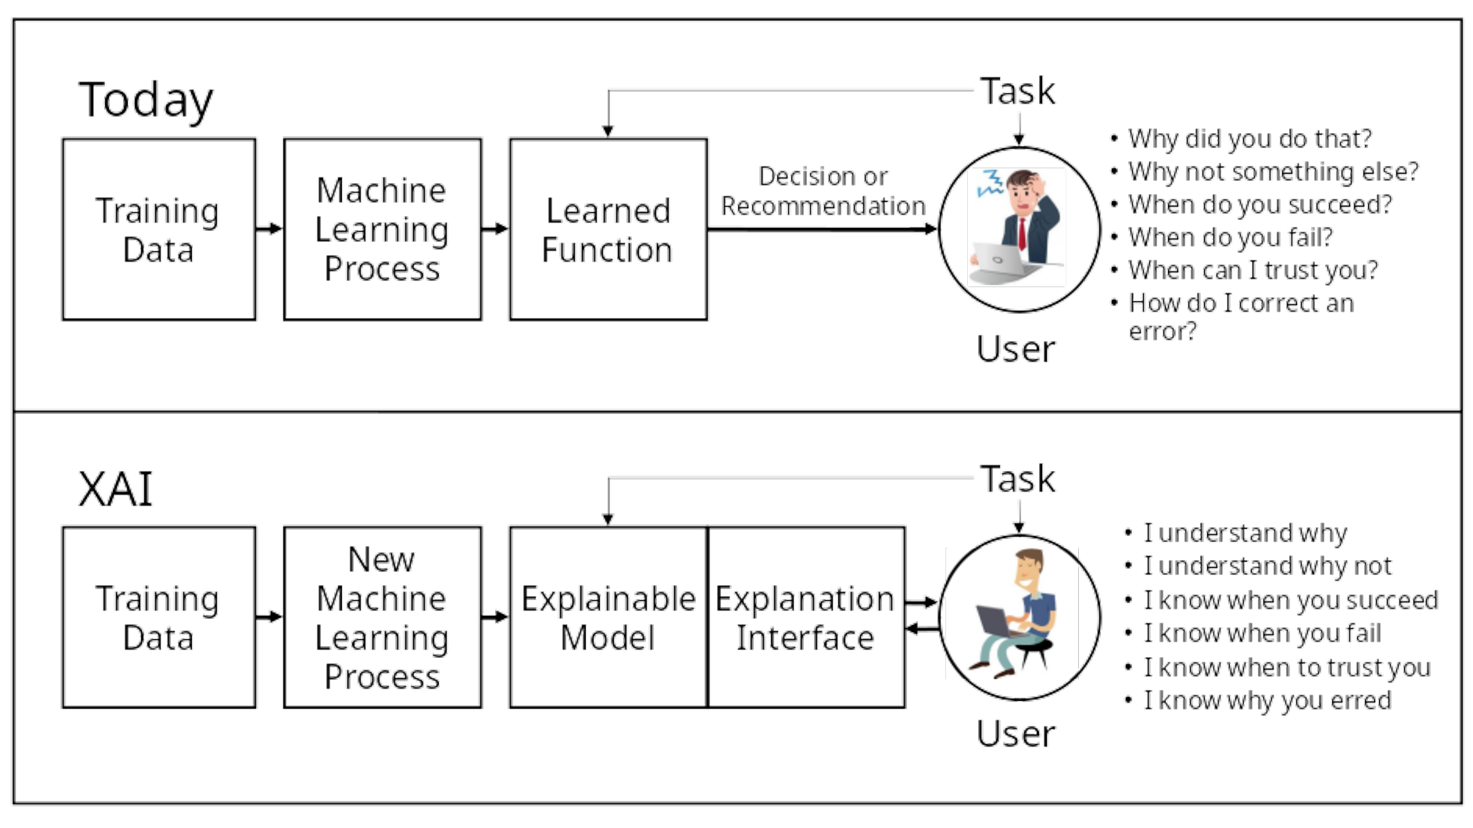
\includegraphics[width=\linewidth]{figures/xai-concept.pdf}
    \end{center}
\end{frame}

%===============================================================================
\section{Background}
%===============================================================================

\subsection{Overview on XAI}

\begin{frame}[allowframebreaks]{Explain What?}
    \begin{block}{Most efforts are devoted to \textbf{supervised} ML, and in particular:}
        \begin{itemize}
            \item specific sorts of \alert{tasks}, e.g. classification and regression
            
            \item specific sorts of \alert{data}, e.g. images, text, or tables 
            
            \item specific sorts of \alert{predictors}, e.g. neural networks, SVM
            %
            \begin{itemize}
                \item[ie] essentially, functions of the form $f: \mathcal{X} \subseteq \mathbb{R}^n \rightarrow \mathcal{Y} \subseteq \mathbb{R}^m$
            \end{itemize}
        \end{itemize}
    \end{block}
    
    \framebreak

    Interpretability--Predictivity trade-off:
    %
    \begin{figure}
        \centering
        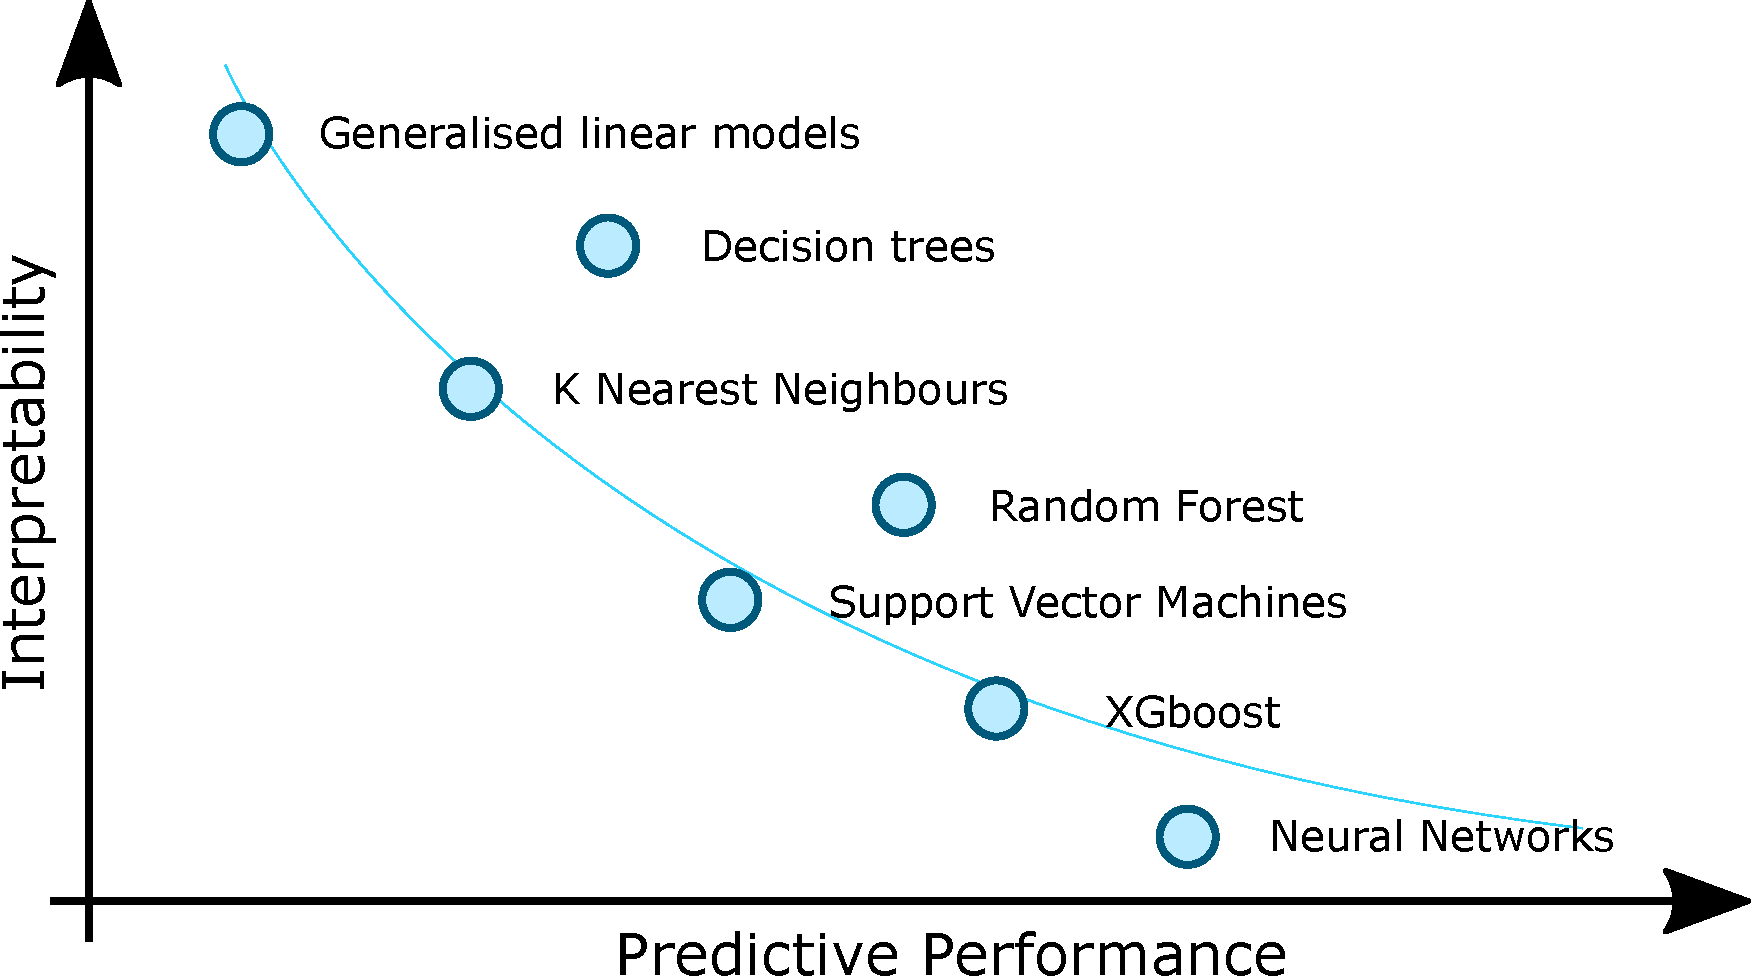
\includegraphics[width=.7\linewidth]{figures/interpretability-performance-tradeoff.pdf}
    \end{figure}

    \framebreak

    \begin{alertblock}{Conventionally\ldots}
        \begin{itemize}
            \item \ldots (generalised) linear models, or decision trees/rules are \alert{considered} interpretable
            \item \ldots other kinds of predictors are considered \alert{poorly} interpretable
            %
            \begin{itemize}
                \item hence needing \alert{explanations}
            \end{itemize}
        \end{itemize}
    \end{alertblock}
    
\end{frame}

\begin{frame}[allowframebreaks]{Global vs. Local Explanations}
    \begin{block}{Global Explanation}
        \begin{itemize}
            \item How does a predictor produces its outcomes in general?
            %
            \begin{itemize}
                \item[eg] how does a neural network classify animals?
            \end{itemize}
        \end{itemize}
    \end{block}

    \begin{block}{Local Explanation}
        \begin{itemize}
            \item How did a predictor produce a particular outcome?
            %
            \begin{itemize}
                \item[eg] why did the neural network classify a cat?
            \end{itemize}
        \end{itemize}
    \end{block}

    \framebreak

    \begin{alertblock}{About the global/local dichotomy}
        \begin{itemize}
            \item firstly introduced in \cite{Ribeiro0G16}
            \item along with \lime{}, i.e. one of the most successful XAI techniques
        \end{itemize}
    \end{alertblock}

    \framebreak

    \begin{figure}
        \centering
        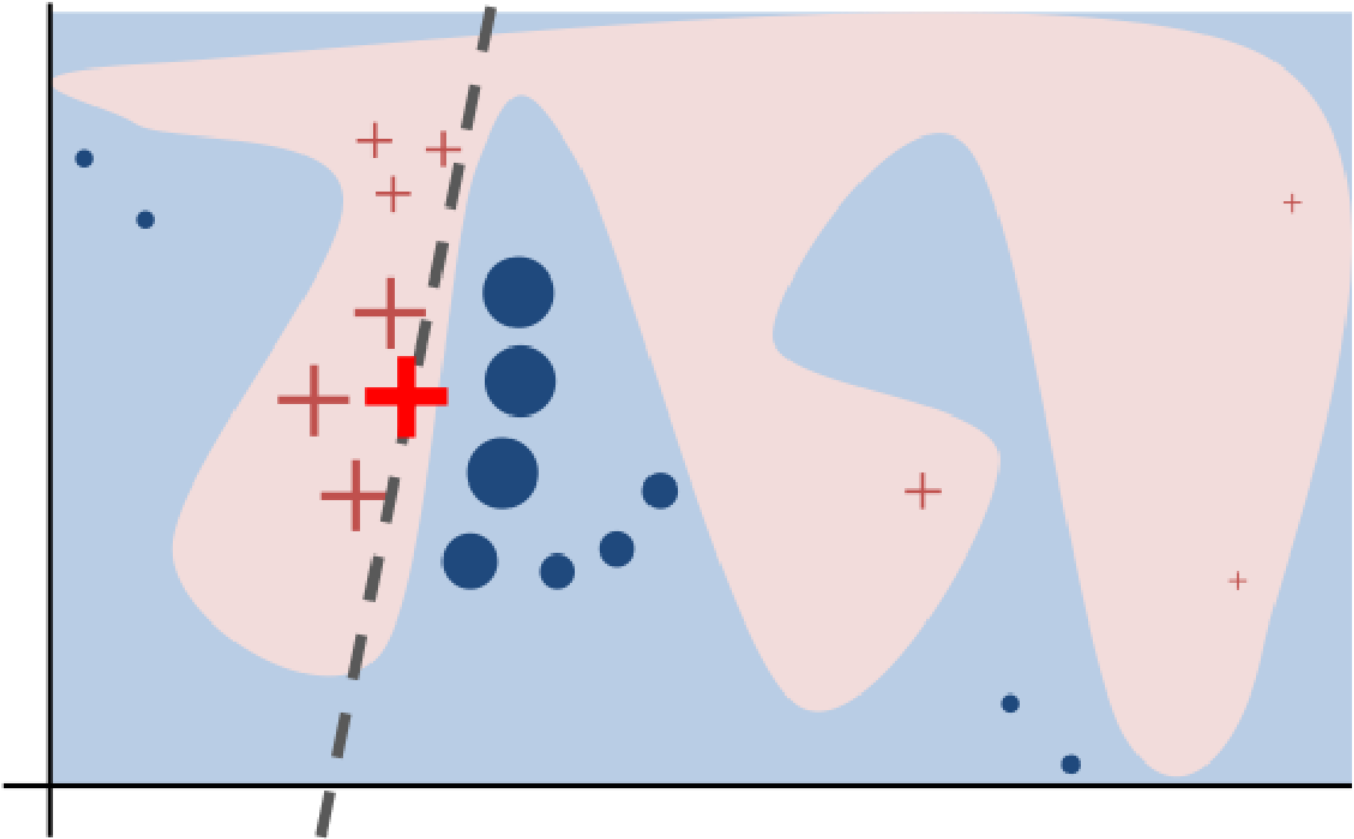
\includegraphics[width=.6\linewidth]{figures/lime.png}
        \caption{(from \cite{Ribeiro0G16}) 
Toy example to present intuition for \lime{}.
The black-box model’s complex decision function $f$ (unknown to \lime{}) is represented by the blue/pink background, which cannot be approximated well by a linear model.
The bold red cross is the instance being explained.
\lime{} samples instances, gets predictions using $f$, and weighs them by the proximity to the instance being explained (represented here by size).
The dashed line is the learned explanation that is locally (but not globally) faithful.
}
    \end{figure}
\end{frame}

\begin{frame}[allowframebreaks]{Overview on XAI approaches}
    Four major approaches, according to \cite{guidotti2018survey}:
    %
    \begin{center}
        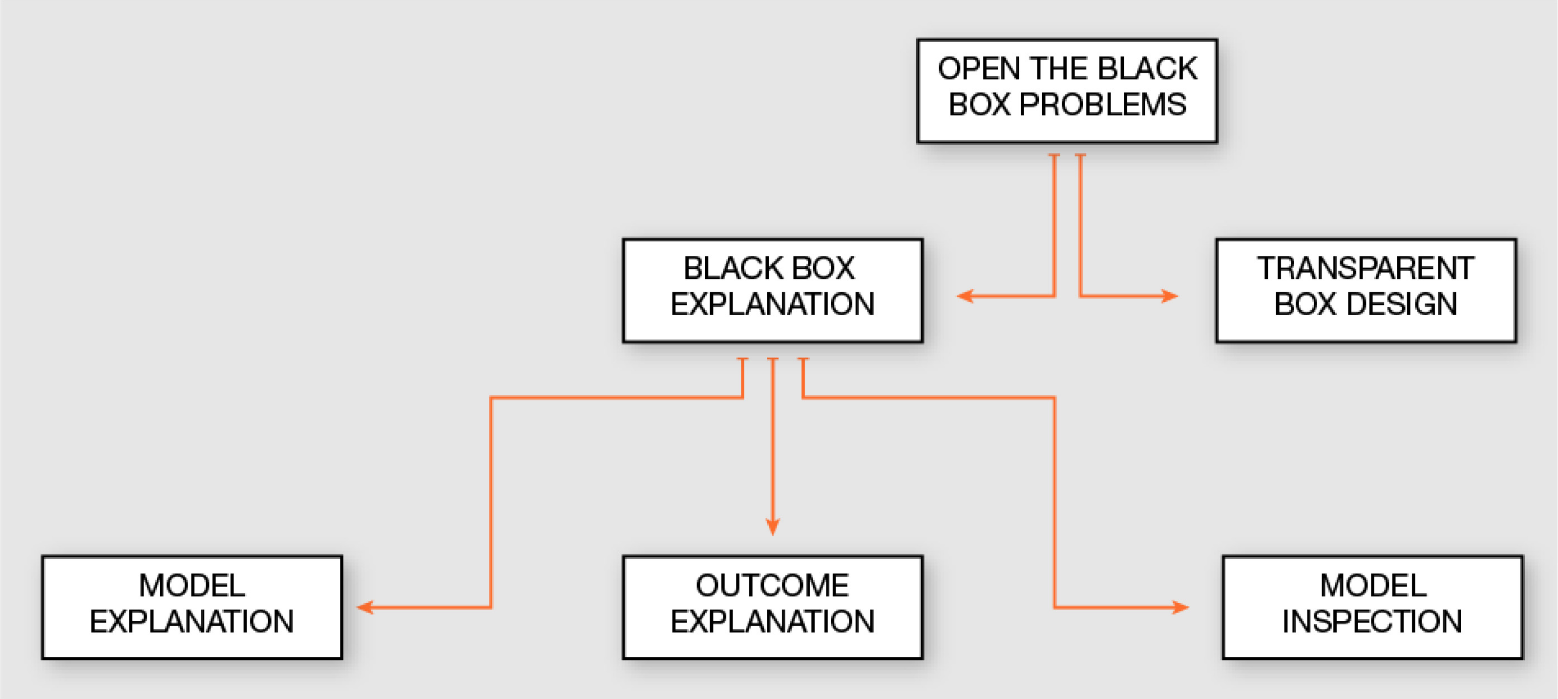
\includegraphics[width=.8\linewidth]{figures/open-bb.png}
    \end{center}

    \begin{block}{About notation}
        \begin{itemize}
            \item ``model'' $\approx$ ``predictor''
        \end{itemize}
    \end{block}
    
    \framebreak

    \begin{block}{Model Explanation ($\approx$ global explanation)}
        \begin{description}
            \item[explanation] $\approx$ interpretable predictor trained to mimic the one to be explained 
            %
            \begin{itemize}
                \item w.r.t. the entire input space
                %
                \begin{itemize}
                    \item[eg] surrogate models (e.g. decision trees)
                \end{itemize}
            \end{itemize}
        \end{description}
    \end{block}
    %
    \begin{center}
        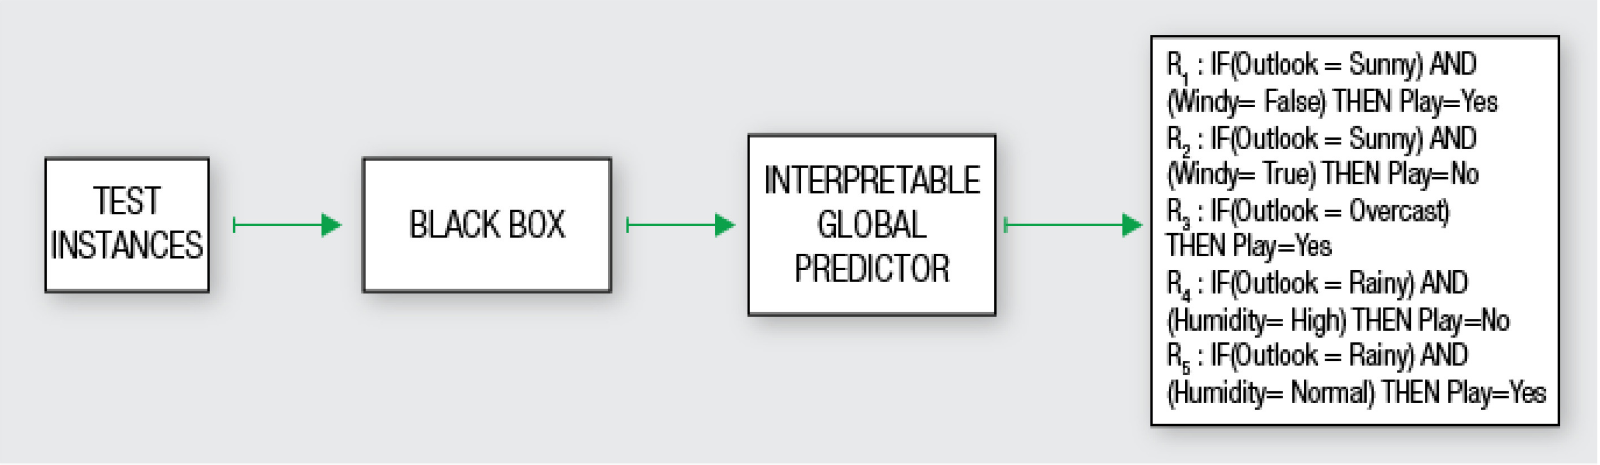
\includegraphics[width=.8\linewidth]{figures/model-explanation.png}
    \end{center}

    \framebreak

    \begin{block}{Outcome Explanation ($\approx$ local explanation)}
        \begin{description}
            \item[explanation] $\approx$ interpretable predictor trained to mimic the one to be explained
            %
            \begin{itemize}
                \item w.r.t. a small portion of the input space
                %
                \begin{itemize}
                    \item[eg] saliency maps (e.g. \lime{}\ccite{Ribeiro0G16}, SHAP\ccite{LundbergL2017})
                \end{itemize}
            \end{itemize}
        \end{description}
    \end{block}
    %
    \begin{center}
        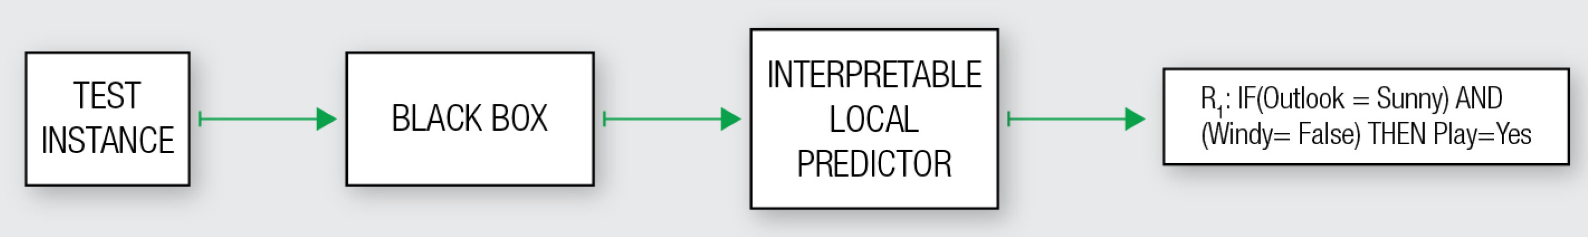
\includegraphics[width=.8\linewidth]{figures/outcome-explanation.png}
    \end{center}

    \framebreak

    \begin{block}{Model Inspection}
        \begin{description}
            \item[explanation] $\approx$ representation summarising the behaviour of the predictor to be explained 
            %
            \begin{itemize}
                \item w.r.t. a given portion of the input space (or, possibly, all of it)
                %
                \begin{itemize}
                    \item[eg] feature importance, sensitivity analysis
                \end{itemize}
            \end{itemize}
        \end{description}
    \end{block}
    %
    \begin{center}
        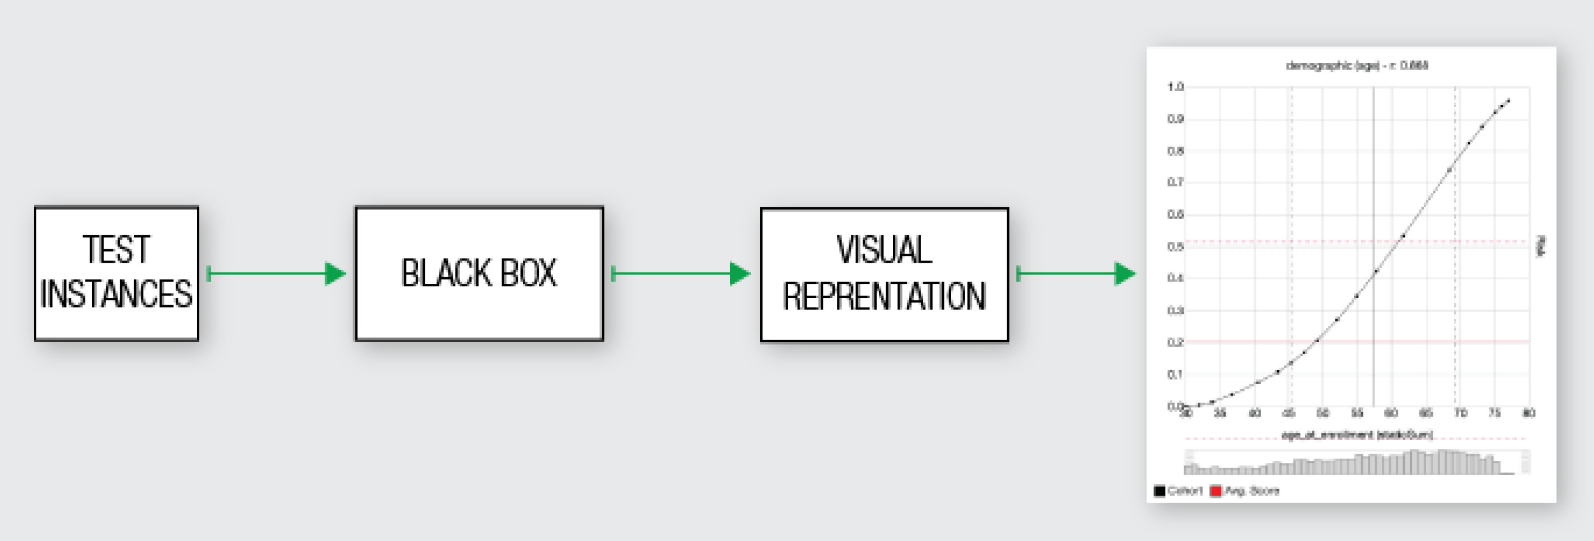
\includegraphics[width=.8\linewidth]{figures/model-inspection.png}
    \end{center}

    \framebreak

    \begin{block}{Transparent Box Design}
        \begin{itemize}
            \item just train an interpretable predictor and look at it
        \end{itemize}
    \end{block}
    %
    \begin{center}
        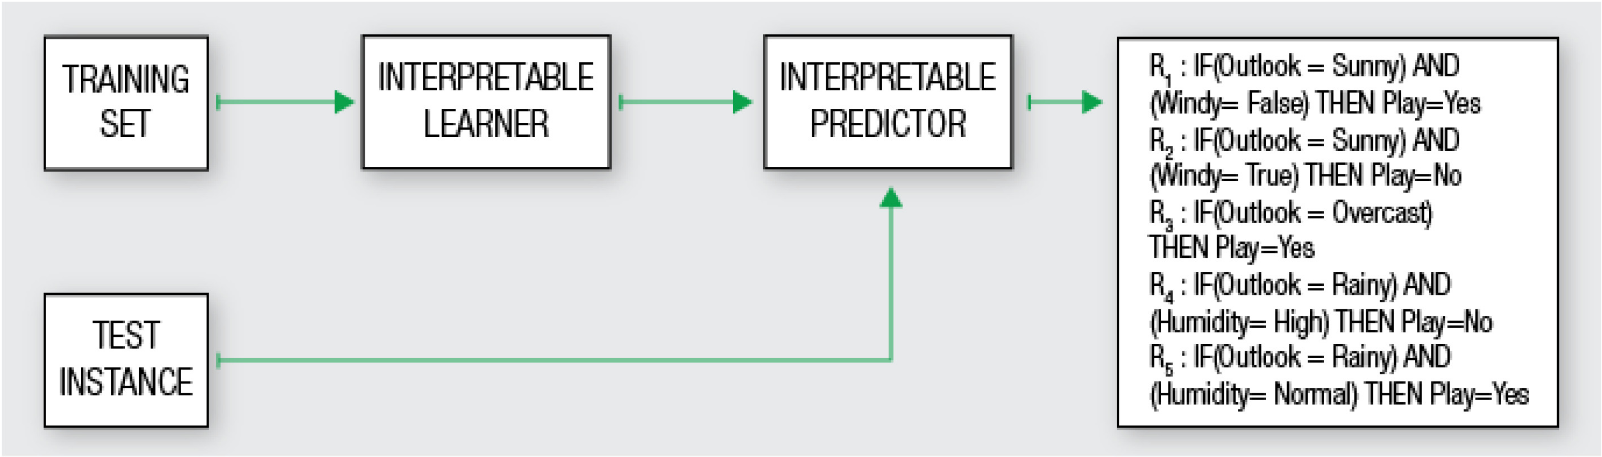
\includegraphics[width=.8\linewidth]{figures/transparent-box-design.png}
    \end{center}
\end{frame}

\subsection{Interpretation vs. Explanation}

\begin{frame}{Interpretation or Explanation?}

    The two terms are \alert{not} interchangeable
    %
    \begin{itemize}
        \item \ldots despite they are often used interchangeably
    \end{itemize}

    \vfill

    \begin{block}{Insights}
        \begin{description}
            \item[interpretation] $\approx$ binding objects with meaning
            %
            \begin{itemize}
                \item that's what the human mind does
            \end{itemize}

            \item[explanation] $\approx$ eliciting relevant aspects of objects (to ease their interpretation)
        \end{description}
    \end{block}
\end{frame}

\begin{frame}{The Role of Representations}

    \begin{center}
        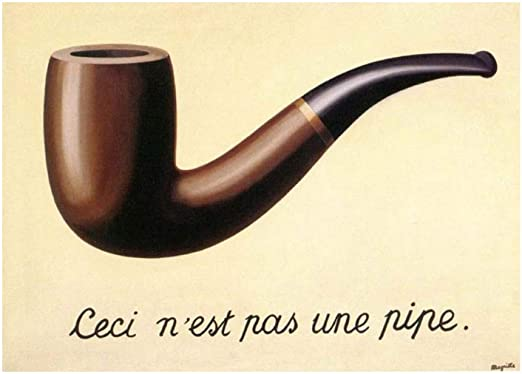
\includegraphics[width=.7\linewidth]{figures/pipe.jpg}
    \end{center}
    %
    \begin{itemize}
        \item[!] this is just a \alert{representation} of a pipe
    \end{itemize}

\end{frame}

\begin{frame}[allowframebreaks]{An abstract framework for XAI\ccite{agentbasedxai-extraamas2020}}

    \begin{center}
        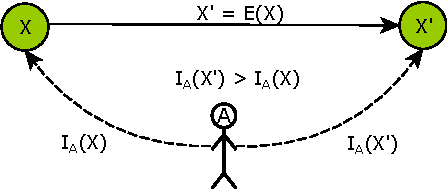
\includegraphics[width=.5\linewidth]{figures/framework.pdf}
    \end{center}
    %
    \begin{itemize}
        \item[$X$] object to be explained
        \item[$A$] observer agent
        \item[$I_A(\cdot)$] a function ``measuring'' the ``degree of interpretability'' of $X$, w.r.t. $A$
        \item[$E(\cdot)$] an \alert{explanation} function, mapping objects into (different) objects      
        \item[$X'$] the \alert{result} of the explanation, i.e. a \alert{more-interpretable} object
    \end{itemize}
    
    \begin{block}{Key points}
        \begin{itemize}
            \item interpretation is \alert{subjective}
            \item explanation is an operation transforming poorly interpretable objects into more-interpretable ones
            \item `interpretability' does not need to be measurable (only comparisons matter)
        \end{itemize}
    \end{block}

    \framebreak

    In the particular case of ML-based AI:
    %
    \begin{center}
        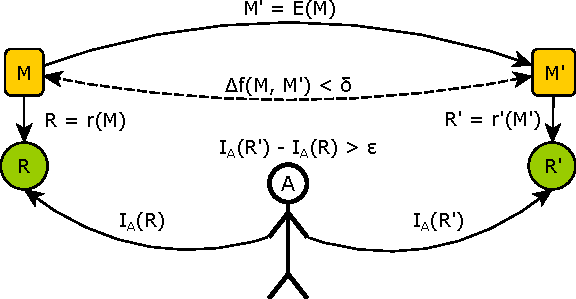
\includegraphics[width=.5\linewidth]{figures/global.pdf}
    \end{center}
    %
    \begin{itemize}
        \item we need to explain a model $M$
        %
        \begin{itemize}
            \item having a poorly interpretable \alert{representation} $R$ (w.r.t. $A$)
        \end{itemize}

        \item explanation produces another model $M'$
        %
        \begin{itemize}
            \item having an interpretable \alert{representation} $R'$ (w.r.t. $A$)
        \end{itemize}

        \item performance difference among $M$ and $M'$ (i.e. $\Delta f(M, M')$) must be small ($< \delta$)
        %
        \begin{itemize}
            \item or, dually, $M'$ must have an high \alert{fidelity} w.r.t. $M$
        \end{itemize}
    \end{itemize}

    \begin{block}{Key points}
        \begin{itemize}
            \item explanation $\approx$ search of a \alert{surrogate} interpretable model
            \item \alert{representation} is important as much as explanation
            \item explanation must maximise \alert{fidelity}
        \end{itemize}
    \end{block}

\end{frame}

\subsection{Explanations via Symbolic Knowledge Extraction}

\begin{frame}[allowframebreaks]{Overview}
    \begin{columns}
        \begin{column}{0.19\linewidth}
            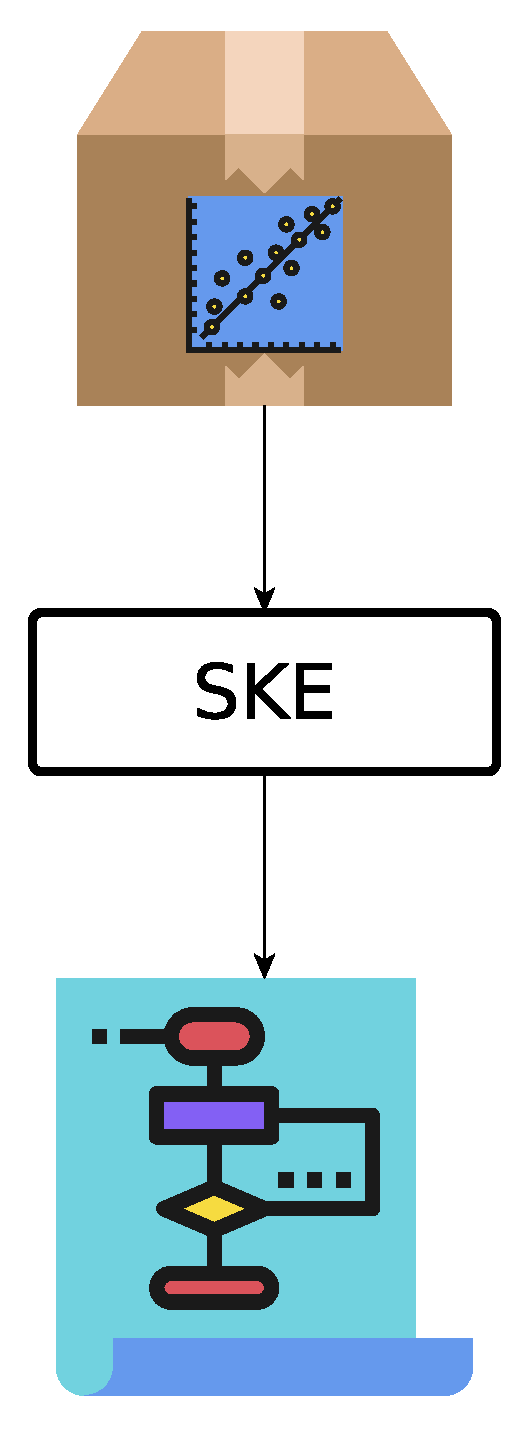
\includegraphics[width=\linewidth]{figures/ske.pdf}
        \end{column}
        \hfill
        \begin{column}{0.8\linewidth}
            \begin{block}{Insight}
                \begin{itemize}
                    \item search of a \alert{surrogate} interpretable model\ldots
                    \medskip
                    \item \ldots consisting of \alert{symbolic knowledge}
                \end{itemize}
            \end{block}
        \end{column}
    \end{columns}

    \framebreak

    \begin{block}{Definition: Symbolic Knowledge Extraction (SKE)}\centering\itshape
        Any \emph{algorithmic} procedure accepting \emph{trained} sub-symbolic predictors as input and producing \emph{symbolic} knowledge as output, in such a way that the extracted knowledge reflects the behaviour of the predictor with high \emph{fidelity}.
    \end{block}
\end{frame}

\begin{frame}[allowframebreaks]{What does `symbolic' actually mean?}
    According to \cite{Gelder90}, \alert{symbolic} representations of knowledge
    %
    \begin{itemize}
        \item involve a \alert{set of symbols},
        \item which can be combined (e.g., concatenated) in (possibly) \alert{infinitely many} ways, 
        \item following precise \alert{syntactical} rules, and
        \item where both elementary symbols and any admissible combination of them can be assigned with \alert{meaning}
        %
        \begin{itemize}
            \item[ie] \alert{each} symbol can be mapped into some entity from the domain at hand.
        \end{itemize}
    \end{itemize}
    
    \begin{exampleblock}{Notable example}
        \begin{itemize}
            \item formal logic
        \end{itemize}
    \end{exampleblock}

    \framebreak

    \begin{alertblock}{Opposite notion: \textbf{distributed} representations}
        \begin{itemize}
            \item where symbols \alert{alone} have no meaning
            \item unless it is considered along with its \alert{neighbourhood}
            %
            \begin{itemize}
                \item[ie] any other symbol which is \alert{close} (according to some notion of closeness)
            \end{itemize}
        \end{itemize}
    \end{alertblock}
\end{frame}

\begin{frame}[allowframebreaks]{Plenty of SKE methods from the literature}
    % !TeX root = ../ise-lab-ske.tex

\newcommand{\myhead}{
	\textbf{\#} & \textbf{Method} & \textbf{Translucency} & \textbf{Task} & \textbf{Input} & \textbf{Expressiveness} & \textbf{Shape} 
    \\\hline\hline
}

\newcounter{SkeMethod}
\setcounter{SkeMethod}{1}
\newcommand{\newSkeMethodIndex}{\theSkeMethod\stepcounter{SkeMethod}}

\begin{scriptsize}
\begin{longtable}{c|p{3cm}|c|c|c|c|c}
    % first header
    \caption{
        Summary of the knowledge-extraction algorithms.
        %
        Symbol $*$ means that the related dimension of the algorithm is not bounded.
        %
        Symbol $\dagger$ means that the output is a power law.
    }
    \label{tab:ske-taxonomy}
    \\
    \myhead
    %
    \newSkeMethodIndex & \cite{breiman1984classification} & P & C+R & C+D & P & DT 
    \\\hdashline
    \newSkeMethodIndex & \cite{Quinlan86ID3} & P & C & D & P & DT 
    \\\hdashline
    \newSkeMethodIndex & \cite{SaitoN88} & P & C & D & P & L 
    \\\hdashline
    \newSkeMethodIndex & \cite{ClarkN89} & P & C & C+D & P & L 
    \\\hline
    \newSkeMethodIndex & \cite{Masuoka1990} & D (NN) & C & C & F & L 
    \\\hdashline
    \newSkeMethodIndex & \cite{Hayashi90} & D (NN) & C & B & F & L 
    \\\hdashline
    \newSkeMethodIndex & \cite{TowellS91} & D (NN) & C & D & MN & L 
    \\\hdashline
    \newSkeMethodIndex & \cite{Berenji91} & D (NN) & C & C & F & L 
    \\\hdashline
    \newSkeMethodIndex & \cite{BrunkP91} & P & C & C+D & P & L 
    \\\hdashline
    \newSkeMethodIndex & \cite{murphy1991id2} & P & C & D & MN & DT 
    \\\hdashline
    \newSkeMethodIndex & \cite{HorikawaFU92} & D (NN) & C & C & F & L 
    \\\hdashline
    \newSkeMethodIndex & \cite{TrespHA92} & D (NN) & R & C & P & L 
    \\\hdashline
    \newSkeMethodIndex & \cite{towell1993extracting} & D (NN) & C & D & P & L 
    \\\hdashline
    \newSkeMethodIndex & \cite{Thrun1993ExtractingPC} & D (NN) & C & C & P+MN & L 
    \\\hdashline
    \newSkeMethodIndex & \cite{Cohen93} & P & C & C+D & P & L 
    \\\hdashline
    \newSkeMethodIndex & \cite{quinlan1993c4} & P & C & C+D & P & DT 
    \\\hdashline
    \newSkeMethodIndex & \cite{Fu94} & D (NN) & C & D & P & L 
    \\\hdashline
    \newSkeMethodIndex & \cite{halgamuge1994neural} & D (NN) & C & C & F & L 
    \\\hdashline
    \newSkeMethodIndex & \cite{MITRA1994285} & D (NN) & C & C+D & F & L 
    \\\hdashline
    \newSkeMethodIndex & \cite{craven1994using} & P & C & B & P+MN & L 
    \\\hdashline
    \newSkeMethodIndex & \cite{FurnkranzW94} & P & C & D & P & L 
    \\\hdashline
    \newSkeMethodIndex & \cite{sestito94automated} & P & C & C & P & L 
    \\\hline
    \newSkeMethodIndex & \cite{Andrews95rulex} & D (NN) & C & C+D & P & L 
    \\\hdashline
    \newSkeMethodIndex & \cite{Matthews95fuzzy} & D (NN) & C & B & F & L 
    \\\hdashline
    \newSkeMethodIndex & \cite{Cohen95} & P & C & C+D & P & L 
    \\\hdashline
    \newSkeMethodIndex & \cite{PopTHSD95} & P & C & B & P & L 
    \\\hdashline
    \newSkeMethodIndex & \cite{SetionoL96} & D (NN) & C & B & P & L 
    \\\hdashline
    \newSkeMethodIndex & \cite{tickle1996dedec} & P & C & B & P & L 
    \\\hdashline
    \newSkeMethodIndex & \cite{YuanZ96} & P & C & D & F & L 
    \\\hdashline
    \newSkeMethodIndex & \cite{craven1996extracting} & P & C & B & P+MN & DT 
    \\\hdashline
    \newSkeMethodIndex & \cite{HongL96} & P & C & C & F & L 
    \\\hdashline
    \newSkeMethodIndex & \cite{Setiono97NeuroLinear} & D (NN3) & C & C+D & O & L 
    \\\hdashline
    \newSkeMethodIndex & \cite{Setiono97a} & D (NN) & C & D & P & L 
    \\\hdashline
    \newSkeMethodIndex & \cite{NauckK97} & D (NN) & C & D & F & L 
    \\\hdashline
    \newSkeMethodIndex & \cite{SaitoN97} & D (NN) & R & C & $\dagger$ & $\dagger$ 
    \\\hdashline
    \newSkeMethodIndex & \cite{BenitezCR97} & D (NN) & C+R & C & F & L 
    \\\hdashline
    \newSkeMethodIndex & \cite{IshibuchiNM97} & P & C & C & F & L 
    \\\hdashline
    \newSkeMethodIndex & \cite{TahaG99} & D (NN) & C & C & P & L 
    \\\hdashline
    \newSkeMethodIndex & \cite{TahaG99} & D (NN) & C & C & P & L 
    \\\hdashline
    \newSkeMethodIndex & \cite{Krishnan99combo} & D (NN) & C & B & P & L 
    \\\hdashline
    \newSkeMethodIndex & \cite{NauckK99} & D (NN) & R & D & F & L 
    \\\hdashline
    \newSkeMethodIndex & \cite{TahaG99} & P & C & B & P & L 
    \\\hdashline
    \newSkeMethodIndex & \cite{KrishnanSB99} & P & C & C & P & DT 
    \\\hdashline
    \newSkeMethodIndex & \cite{schmitz1999NN} & P & C+R & C+D & P & DT 
    \\\hdashline
    \newSkeMethodIndex & \cite{HongC99} & P & C & C & F & L 
    \\\hline
    \newSkeMethodIndex & \cite{Setiono00} & D (NN) & C & B & MN & L 
    \\\hdashline
    \newSkeMethodIndex & \cite{Tsukimoto00} & D (NN) & C & C+D & P & L 
    \\\hdashline
    \newSkeMethodIndex & \cite{Kim2000} & D (NN4) & C & C+D & P & DT 
    \\\hdashline
    \newSkeMethodIndex & \cite{SetionoL00} & D (NN) & R & C+D & P+MN+O & DT 
    \\\hdashline
    \newSkeMethodIndex & \cite{ZhouCC00} & P & C & C+D & P & L 
    \\\hdashline
    \newSkeMethodIndex & \cite{HongC00a} & P & C & C & F & L 
    \\\hdashline
    \newSkeMethodIndex & \cite{sato2001rule} & D (NN3) & R & C+D & P & DT 
    \\\hdashline
    \newSkeMethodIndex & \cite{parpinelli2001ant} & P & C & C+D & P & L 
    \\\hdashline
    \newSkeMethodIndex & \cite{CastilloGP01} & P & C+R & C+D & F & L 
    \\\hdashline
    \newSkeMethodIndex & \cite{saito2002extracting} & D (NN) & R & C+D & P & L 
    \\\hdashline
    \newSkeMethodIndex & \cite{setiono2002extraction} & D (NN3) & R & C+D & P & L 
    \\\hdashline
    \newSkeMethodIndex & \cite{liu2002density} & P & C & C+D & P & L 
    \\\hdashline
    \newSkeMethodIndex & \cite{Boz02} & P & C & C+D & P & DT 
    \\\hdashline
    \newSkeMethodIndex & \cite{Markowska-KaczmarT03} & P & C & C+D & F & L 
    \\\hdashline
    \newSkeMethodIndex & \cite{ZhouJC03} & P & C & C+D & P & L 
    \\\hdashline
    \newSkeMethodIndex & \cite{SetionoT04} & D (NN3) & R & C+D & P & L 
    \\\hdashline
    \newSkeMethodIndex & \cite{Fu2004} & D (SVM) & C & C+D & P & L 
    \\\hdashline
    \newSkeMethodIndex & \cite{Markowska-KaczmarC04} & P & C & C+D & P & L 
    \\\hdashline
    \newSkeMethodIndex & \cite{RabunalDPPR04} & P & C & C+D & P & L 
    \\\hdashline
    \newSkeMethodIndex & \cite{Chen2004LEARNINGAA} & P & C & C & P & L 
    \\\hdashline
    \newSkeMethodIndex & \cite{LiuAM04} & P & C & C+D & P & L 
    \\\hdashline
    \newSkeMethodIndex & \cite{Browne2004} & P & C & C+D & P+MN & DT 
    \\\hline
    \newSkeMethodIndex & \cite{ZhangSJC05} & D (SVM) & C & C & P & L 
    \\\hdashline
    \newSkeMethodIndex & \cite{barakat2005eclectic} & D (SVM) & C+R & * & * & * 
    \\\hdashline
    \newSkeMethodIndex & \cite{FungSR05} & D (SVM+LC) & C & C & P & L 
    \\\hdashline
    \newSkeMethodIndex & \cite{ChavesVT05} & D (SVM) & C & C & F & L 
    \\\hdashline
    \newSkeMethodIndex & \cite{Torres2005} & P & C & C+D & P+MN & DT 
    \\\hdashline
    \newSkeMethodIndex & \cite{EtchellsL06} & P & C & C+D & P & L 
    \\\hdashline
    \newSkeMethodIndex & \cite{He2006} & P & C & C+D & P & DT 
    \\\hdashline
    \newSkeMethodIndex & \cite{huysmans2006iter} & P & R & C & P & L 
    \\\hdashline
    \newSkeMethodIndex & \cite{BaderHM07} & D (NN) & C & B & P & L 
    \\\hdashline
    \newSkeMethodIndex & \cite{SchetininFPCKEBH07} & D (DTE) & R & C & P & DT 
    \\\hdashline
    \newSkeMethodIndex & \cite{ChenLW07} & D (SVM) & C & C & P & L 
    \\\hdashline
    \newSkeMethodIndex & \cite{BarakatB07} & D (SVM) & C & C+D & P & L 
    \\\hdashline
    \newSkeMethodIndex & \cite{SaadW07} & P & C & C+D & O & L 
    \\\hdashline
    \newSkeMethodIndex & \cite{MartensBHVSB07} & P & C & C+D & P & L 
    \\\hdashline
    \newSkeMethodIndex & \cite{NunezAC08} & D (SVM) & C & C & P+O & L 
    \\\hdashline
    \newSkeMethodIndex & \cite{SetionoBM08} & P & C & C+D & P+O & L
    \\\hdashline
    \newSkeMethodIndex & \cite{OdajimaHTS08} & P & C & D & P & L 
    \\\hdashline
    \newSkeMethodIndex & \cite{grex-icdm2008} & P & C+R & C+D & F & DT 
    \\\hdashline
    \newSkeMethodIndex & \cite{Bader09} & D (NN) & C & B & P & L 
    \\\hdashline
    \newSkeMethodIndex & \cite{MartensBG09} & D (SVM) & C & * & * & * 
    \\\hline
    \newSkeMethodIndex & \cite{LehmannBH10} & P & C & B & P & L 
    \\\hdashline
    \newSkeMethodIndex & \cite{AugastaK12} & P & C & C+D & P & L 
    \\\hdashline
    \newSkeMethodIndex & \cite{sethi2012kdruleex} & P & C & C+D & P & TA 
    \\\hline
    \newSkeMethodIndex & \cite{ZilkeMJ16} & D (NN) & R & C+D & P & DT 
    \\\hdashline
    \newSkeMethodIndex & \cite{ChanC17} & D (NN) & R & C & P & L 
    \\\hdashline
    \newSkeMethodIndex & \cite{YedjourB18} & P & C & B & P & L 
    \\\hdashline
    \newSkeMethodIndex & \cite{CHAN2020329} & D (NN) & R & C & P & L 
    \\\hline
    \newSkeMethodIndex & \cite{WangWWYWJ20} & D (DTE) & C & C & P & L 
    \\\hdashline
    \newSkeMethodIndex & \cite{gridex-extraamas2021} & P & R & C & P & L 
\end{longtable}
\end{scriptsize}

% Regex per togliere gli acronimi (incompleta al momento)
% ([a-z]|[A-Z]|\\|[0-9]|\{|\}| |\.|\-|\+|\[|\])* &

\end{frame}

\begin{frame}[allowframebreaks]{Taxonomy of SKE methods}
    \begin{center}
        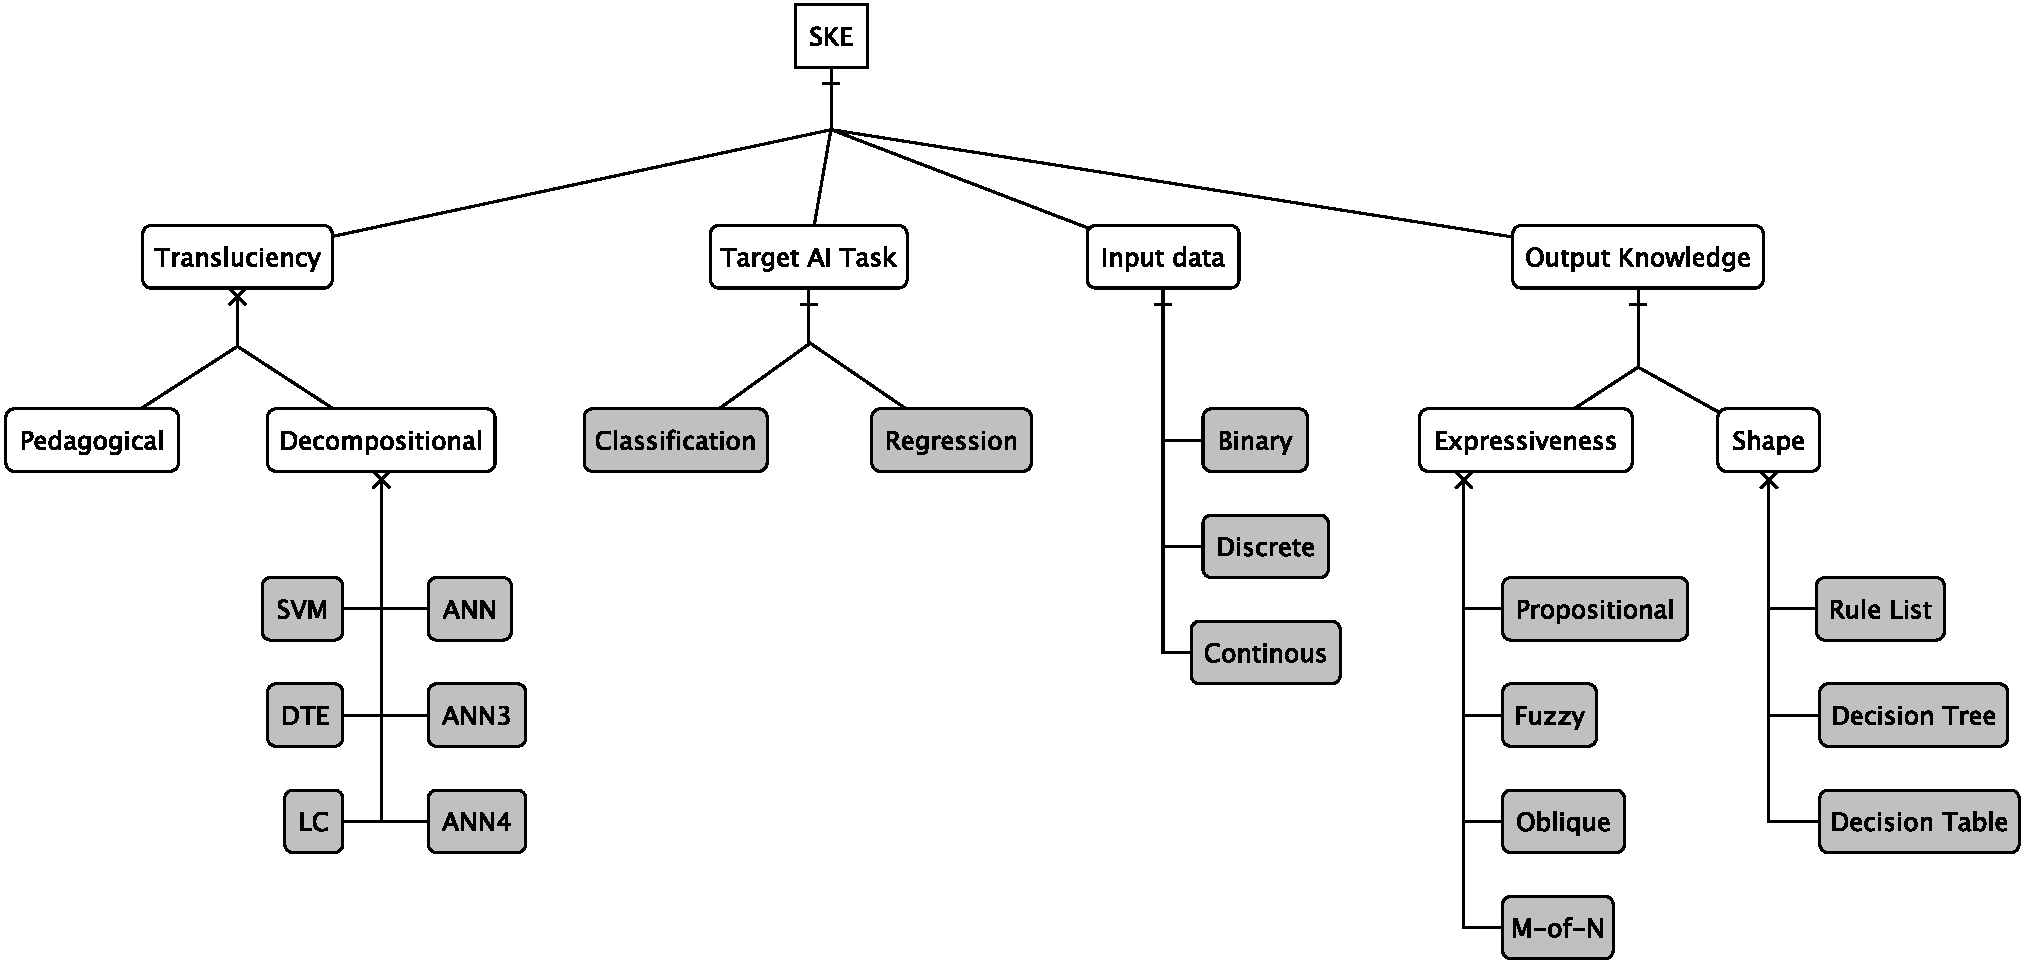
\includegraphics[width=\linewidth]{figures/ske-taxonomy.pdf}
    \end{center}
    
    \framebreak

    \begin{description}
        \item[target AI task] for the predictor undergoing extraction
        %
        \begin{description}
            \item[classification] i.e., $f: \mathcal{X} \subseteq \mathbb{R}^n \rightarrow \mathcal{Y}$ s.t. $|\mathcal{Y}| = k$
            \item[regression] i.e., $f: \mathcal{X} \subseteq \mathbb{R}^n \rightarrow \mathcal{Y} \subseteq \mathbb{R}^m$     
        \end{description} 

        \medskip

        \item[translucency] what kind of ML predictor does the SKE method support?
        %
        \begin{description}
            \item[pedagogical:] any supervised predictor
            \item[decompositional:] a particular sort of ML predictor (e.g. NN, SVM, DT)      
        \end{description} 

        \medskip

        \item[input data] supported by the predictor undergoing extraction
        %
        \begin{description}
            \item[binary:] $\mathcal{X} \equiv \{0, 1\}^n$
            \item[discrete:] $\mathcal{X} \in \{x_1, \ldots, x_n\}^n$   
            \item[continuous:] $\mathcal{X} \subseteq \mathbb{R}^n$     
        \end{description} 

        \medskip

        \item[shape] of the extracted knowledge
        %
        \begin{description}
            \item[rule list] i.e. ordered sequences of if-then-else rules
            \item[decision tree] hierarchical set of if-then-else rules involving a comparison among a variable and a constant   
            \item[decision table:] TBD
        \end{description} 

        \medskip

        \item[expressiveness] of the extracted knowledge
        %
        \begin{description}
            \item[propositional] i.e. ordered sequences of if-then-else rules
            \item[fuzzy] hierarchical set of if-then-else rules involving a comparison among a variable and a constant   
            \item[oblique] TBD
            \item[M-of-N] 
        \end{description} 

    \end{description}
\end{frame}

\begin{frame}{Examples of methods and their classification}
    \begin{itemize}
        \item 
    \end{itemize}
\end{frame}

%===============================================================================
\section{A Platform for Symbolic Knowledge Extraction}
%===============================================================================

\begin{frame}{Overall Design}
    \begin{itemize}
        \item 
    \end{itemize}
\end{frame}

\begin{frame}{API Design}
    \begin{itemize}
        \item 
    \end{itemize}
\end{frame}

\begin{frame}{About the extracted knowledge}
    \begin{itemize}
        \item classification problems
        \item regression problems
    \end{itemize}
\end{frame}

\subsection{Usage Examples}

\begin{frame}{Iris (classification)}
    \begin{itemize}
        \item 
    \end{itemize}
\end{frame}

\begin{frame}{Combined Cycle Power Plant (regression)}
    \begin{itemize}
        \item 
    \end{itemize}
\end{frame}

%===============================================================================
\section{Discussion}
%===============================================================================

\begin{frame}{Notable Remarks}
    \begin{itemize}
        \item commitment to a particular output shape / expressiveness
        %
        \begin{itemize}
            \item to preserve both human- and machine-interpretability
            \item other syntaxes may exist
        \end{itemize}
        \item discretization of the input space
        \item discretization of the output space
        \item features should have semantics per se
        \item further refinements may be applied to rules
        \item rules constitute global explanations
    \end{itemize}
\end{frame}

\begin{frame}{Current Limitations}
    \begin{itemize}
        \item tabular data as input $\rightarrow$ doesn't really work with images
        \item high dimensional datasets $\rightarrow$ very large, poorly readable rules
        \item highly variable input spaces $\rightarrow$ many rules $\rightarrow$ poor readability
    \end{itemize}
\end{frame}

\begin{frame}{Future research activities}
    \begin{itemize}
        \item target images or highly dimensional data in general
        \item target reinforcement learning (when based on NN)
        \item target unsupervised learning
        \item design and prototype your own extraction algorithm
    \end{itemize}
\end{frame}

%===============================================================================
\section*{}
%===============================================================================

%/////////
\frame{\titlepage}
%/////////

%===============================================================================
\section*{\refname}
%===============================================================================

%%%%
\setbeamertemplate{page number in head/foot}{}
%/////////
% \begin{frame}[c,noframenumbering]{\refname}
\begin{frame}[t,allowframebreaks,noframenumbering]{\refname}
%	\tiny
    \scriptsize
%	\footnotesize
    \bibliographystyle{apalike-AMS}
    \bibliography{ise-lab-ske}
\end{frame}
%/////////

%%%%%%%%%%%%%%%%%%%%%%%%%%%%%%%%%%%%%%%%%%%%%%%%%%%%%%%%%%%%%%%%%%%%%%%%%%%%%%%%
\end{document}
%%%%%%%%%%%%%%%%%%%%%%%%%%%%%%%%%%%%%%%%%%%%%%%%%%%%%%%%%%%%%%%%%%%%%%%%%%%%%%%%
